\chapter{Experimental task 2 - CleaningRobot - \notdd group}
\label{appendix:B_CleaningRobot}
\section{Constraints}
Your project must be free of syntactic errors. Please make sure that your code actually runs in PyCharm.


\section{Task goal}
The goal of this task is to develop a cleaning robot; the robot moves in a room and cleans the dust on the floor along the way. To clean the dust, the robot is equipped with a cleaning system placed underneath it. When the robot is turned on, it turns on the cleaning system.
The robot moves into the room, thanks to two DC motors, one that controls its wheels and another that controls its rotation, by executing a command, which a Route Management System (RMS) sends to the robot. While moving in the room, the robot can encounter obstacles: these can be detected thanks to an infrared (IR) distance sensor placed in the front.
The robot can check the charge left in its internal battery: to do so, it is equipped with an Intelligent Battery Sensor (IBS); furthermore, a recharging LED is mounted on the top of the robot to signal that it needs to be recharged.

The room, where the robot moves, is represented as a rectangular grid with $x$ and $y$ coordinates; the origin cell of the grid - \ie $(0,0)$ - is located in the bottom-left corner. A cell of the grid may or may not contain an obstacle. The RMS keeps track of the room layout, including the position of the last obstacle encountered in the room.
To recap, the following sensors, actuators, and systems are present:

\begin{itemize}
    \item DC motor to control the wheels in order to move the robot forward.
    \item DC motor to control the rotation of the body of the robot, in order to make it rotate left or right.
    \item RMS, sending commands to the robot.
    \item Infrared distance sensor used to detect obstacles.
    \item IBS to determine the battery charge left.
    \item Recharge LED.
    \item Cleaning system.
\end{itemize}

The communication between the main board and the other components happens with GPIO pins; GPIO communication is configured in BOARD mode. For further details on how to use the GPIO library refer to the \texttt{mock.GPIO} file in the source code.
Handle any error situation that you may encounter by throwing the \texttt{CleaningRobotError} exception.
For now, you don't need to know more; further details will be provided in the user stories below.

\section{Instructions}
Depending on your preference, either clone the repository at \url{https://github.com/Espher5/cleaning_robot} or download the source files as a zip archive; afterwards, import the project into PyCharm. 
Take a look at the provided project, which contains the following classes: 
\begin{itemize}
    \item \textbf{\texttt{CleaningRobot}}: you will implement your methods here.
    \item \textbf{\texttt{CleaningRobotError}}: exception that you will raise to handle errors.
    \item \textbf{\texttt{CleaningRobotTest}}: you can write your tests here.
    \item \textbf{\texttt{mock.GPIO}}: contains the mocked methods for GPIO functionalities.
\end{itemize}


Remember, you are not allowed to modify the provided API in any way (\ie class names, method names, parameter types, return types). You can however add fields, methods, or even classes (including other test classes), as long as you comply with the provided API.
Use \notdd to implement this software system (\ie use the development approach you prefer but not \tdd).
The requirements of the software system to be implemented are divided into a set of user stories, which serve as a to-do list; you should be able to incrementally develop the software system, without an upfront comprehension of all the requirements. Do not read ahead and handle the requirements (\ie specified in the user stories) one at a time in the order provided.
When a story is implemented, move on to the next one. A story is implemented when you are confident that your software system correctly implements all the functionality stipulated by the story's requirement. You may need to review your software system as you progress towards more advanced requirements.
At the end of the task, fill out the post-questionnaire where, among other things, you will be asked to share your project (either as a link to a GitHub repository or as a public link to a zip file). The post-questionnaire is available at: \url{https://forms.gle/GEXHybbDJujZJz2V6}.


\section{User Stories}
\subsection{Robot deployment}
The robot has a status, namely a string (without white spaces) formatted as follows: $(x,y,h)$. The pair $(x,y)$ represents the position of the robot in the room (in terms of $x$ and $y$ coordinates) while $h$ is the heading - \ie the direction the robot is pointing towards; the direction can be: $N (North)$, $S (South)$, $E (East)$, or $W (West)$. The robot assumes the $North$ is parallel to the $y$-axis. The robot starts its duty from the origin position - \ie, the position with coordinates $(0,0)$, facing $North$ (see figure \ref{room_and_compass} below).

\begin{figure}[H]
    \centering
    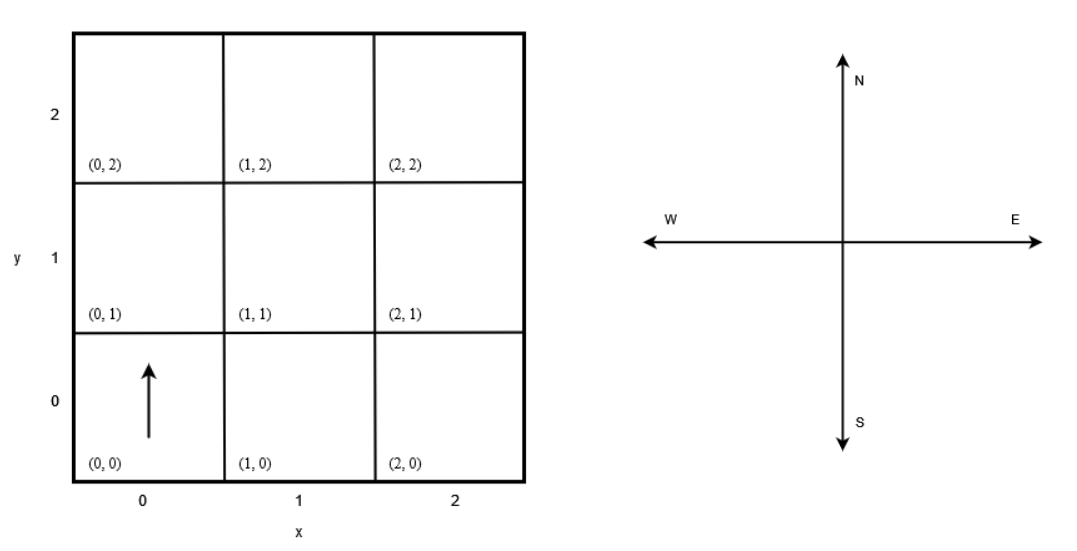
\includegraphics[width=\linewidth]{figures/appendix/cleaning_robot_1.png}
    \caption{Room layout and robot compass.}
    \label{room_and_compass}
\end{figure}

\noindent\textbf{Requirement}:
\begin{itemize}
    \item Implement \texttt{CleaningRobot.initialize\_robot $\,\to\,$ None} to set the status of the robot to "$(0,0,N)$".
    \item Implement \texttt{CleaningRobot.robot\_status()  $\,\to\,$ str} to retrieve the current status of the robot.
\end{itemize}

\noindent\textbf{Example}:
\begin{itemize}
    \item The robot status "$(0,0,N)$" indicates that the robot lies in the cell with $x$ and $y$ coordinates both equal to 0. The heading of the robot is $N$ - \ie it is pointing $North$.
\end{itemize}


\subsection{Robot startup}
When the robot is turned on, it first checks how much battery is left by querying the IBS. If the capacity returned by the IBS is equal to or less than 10\%, the robot turns on the recharging led. Otherwise, the robot turns on the cleaning system and sends its status to the RMS. In any case, the robot stands still.

The IBS is connected on pin 11 (BOARD mode). The communication with the sensor happens via the GPIO \texttt{input} function. For this sensor, the value returned by the GPIO \texttt{input} function is assumed to be a percentage indicating the amount of battery charge left. 
The recharge LED is connected on pin 12 (BOARD mode). The communication with the sensor happens via the GPIO \texttt{output} function.
Finally, the cleaning system is connected on pin 13 (BOARD mode). Assume this component to be an independent system; the communication with it happens via the GPIO \texttt{output} function.
The pin for the IBS, the one for the recharge LED and the one for the cleaning system have already been set up in the constructor of the \texttt{CleaningRobot} class.
Since at this stage of development there is no way to determine the state of the physical LED and cleaning system, use the \texttt{self.battery\_led\_on} and \texttt{self.cleaning\_system\_on} instance variables to keep track of their states.

\noindent\textbf{Requirement}:
\begin{itemize}
    \item Implement \texttt{CleaningRobot.manage\_battery() $\,\to\,$ None} to control the behavior associated with the battery level.
\end{itemize}


\subsection{Robot movement}
To move into the room, the robot must receive a command from the RMS; when this happens, the robot controls the wheel motor and the rotation motor in order to execute the command and finally returns its new status to the RMS.
The robot moves one cell forward when it receives the command "$f$". If the robot receives the command "$r$" or "$l$", it turns right or left respectively - \ie it rotates clockwise or counterclockwise 90$^{\circ}$ around itself. The robot cannot move backwards.
The two motors that control the wheels of the robot and the rotation of the body are DC motors, and the pins to connect them to the main board have already been set up in the constructor of the \texttt{CleaningRobot} class.
In order to control them, please use the following two methods in the \texttt{CleaningRobot} class:
\begin{itemize}
    \item \texttt{activate\_wheel\_motor() $\,\to\,$ None}  activates the wheel motor to make the robot move forward.
    \item \texttt{activate\_rotation\_motor(direction: str) $\,\to\,$ None} activates the rotation motor to make the robot turn left or right, based on the direction parameter ("$l$" to turn left or "$r$" to turn right)
\end{itemize}

\ \\ \
\noindent\textbf{Requirement}:
\begin{itemize}
    \item Implement \texttt{CleaningRobot.execute\_command(command: str) $\,\to\,$ str} to execute the command corresponding to the string given by the RMS and return the status of the robot.
\end{itemize}

\ \\ \
\noindent\textbf{Example}:
\begin{itemize}
    \item If the robot status is "$(0,0,N)$" and it receives the command "$f$", the robot moves one cell forward - \ie the robot controls the wheel motor in order to move one cell forward - and returns the new status "$(0,1,N)$". 
    \item If the status of the robot is "$(0,0,N)$" and it receives the command "$r$", the robot rotates clockwise 90$^{\circ}$ - \ie the robot controls the rotation motor in order to rotate 90$^{\circ}$ - and returns the new status "$(0,0,E)$". Similarly, if it receives the command string "$l$", the robot rotates counterclockwise 90$^{\circ}$ and returns the new status "$(0,0,W)$".
    \item If the  status of the robot is "$(1,1,N)$" and it receives the command "$f$", the robot moves forward and returns the new status "$(1,2,N)$". If the robot receives the command "$l$" afterwards, it turns left and returns the new status "$(1,2,W)$".
\end{itemize}

\noindent\textbf{Hint}:
\begin{itemize}
    \item Remember that you can use the \texttt{robot\_status() $\,\to\,$ str} method in the \texttt{CleaningRobot} class to retrieve the current status of the robot.
    \item Use the class variables provided in the \texttt{CleaningRobot} class to update the rotation of the robot ($N$, $E$, $S$, $W$).
\end{itemize}


\subsection{Obstacle detection}
While executing a command, the robot can encounter an obstacle in a cell;  the robot uses the infrared distance sensor to determine if there is an obstacle in front of it and thus avoid bumping into it. 
If an obstacle is detected, the robot cannot move beyond it; it will instead return its new status, including the positions of the encountered obstacle. In this case, the robot status is a string formatted as follows: "$(x,y,h)(x_o,y_o)$". The triple "$(x,y,h)$" represents the usual position and heading of the robot while the pair "$(x_o,y_o)$" represents the position of the encountered obstacle.
In case multiple commands are executed in sequence, and multiple obstacles are found, the system only keeps track of the last one encountered.

The infrared sensor is connected to the main board on pin 15 (BOARD mode); communication with the sensor happens via the GPIO \texttt{input} function. The pin has already been set up in the constructor of the \texttt{CleaningRobot class}. 
Finally, the output of the infrared sensor is an analog signal which changes intensity according to the distance between the sensor and the object (\ie 2.5V when an object is 50 cm away and ~0V when the object is out of the max range of the sensor). For this exercise, let's assume the input can be classified into just these two categories:
\begin{itemize}
    \item \textbf{Non-zero value}: it indicates that an object is present in front of the sensor (\ie an obstacle).
    \item \textbf{Zero value}: nothing is detected in front of the sensor.
\end{itemize}

\ \\ \
\noindent\textbf{Requirement}:
\begin{itemize}
    \item Implement \texttt{CleaningRobot.obstacle\_found() $\,\to\,$  bool} to determine whether an obstacle is in front of the robot (as detected by the infrared distance sensor).
    \item Update the implementation of \texttt{CleaningRobot.execute\_command(command: str) $\,\to\,$  str} to include the obstacle processing steps.
    \item Update the implementation of \texttt{CleaningRobot.robot\_status() $\,\to\,$  str} to retrieve the current status of the robot, including the possible encountered obstacle.
\end{itemize}

\noindent\textbf{Example}:
\begin{itemize}
    \item Let us suppose that there is an obstacle in the room at coordinates $(0,1)$ (see figure \ref{room_obstacle} below). The robot with initial status "$(0,0,N)$", after executing the command string "$f$", returns the following status: "$(0,0,N)(0,1)$".
\end{itemize}

\begin{figure}[H]
    \centering
    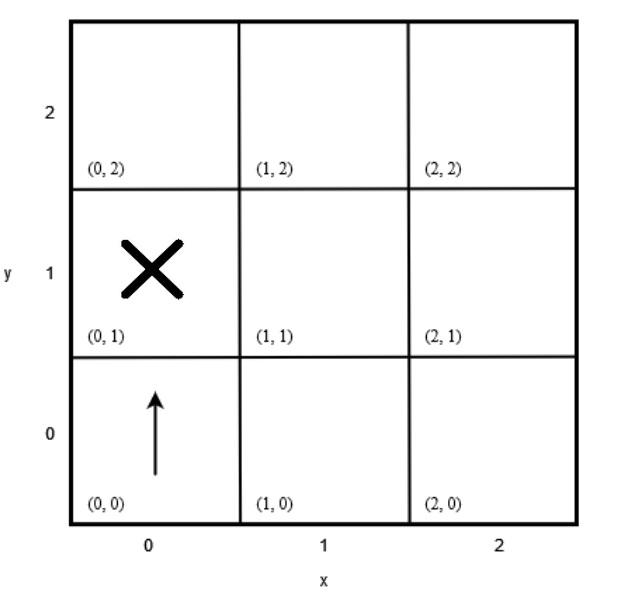
\includegraphics[width=0.5\linewidth]{figures/appendix/cleaning_robot_2.png}
    \caption{Room layout with an obstacle.}
    \label{room_obstacle}
\end{figure}

\noindent\textbf{Hint}:
\begin{itemize}
    \item To keep track of the position of the obstacle after detecting it, use the \texttt{self.obstacle} instance variable in the \texttt{CleaningRobot} class.
\end{itemize}


\subsection{Robot recharge}
Before making any kind of movement/rotation, the robot checks how much battery is left by querying the IBS. When the capacity returned by the IBS is equal to or less than 10\%, the robot shuts down the cleaning system, turns on the recharging led, and stands still (\ie it doesn't update its position in any way).

\noindent\textbf{Requirement}:
\begin{itemize}
    \item Update the implementation of \texttt{CleaningRobot.execute\_command(command: str)  $\,\to\,$ str} to control the behavior associated with the battery level.
    \item Update the implementation of  \texttt{CleaningRobot.manage\_battery()  $\,\to\,$ None} to control the behavior associated with the battery level.
\end{itemize}